\chapter{Project Design}

In this chapter we list the functional requirements of the application with some rudimentary explanations. Using UML(Unified Modeling Language) to identify the users of the application, show possible use cases. Describe the architecture of the application as well as give a layout of the database design and what protocols will be used and why.
\section{Functional Requirements}
\begin{itemize}
\item registration clients
\item enable user logging in and logging out 
\item client offer management - add, edit and remove an offer for a house rental
\item user management - list registered clients and their personal details, revoke users, add users administratively 
\item search function - search offer by set of criteria such as location, price availability 
\item basic booking management - Allow landlords to view forthcoming reservations, confirm clients stay as well as allow clients to make bookings and view forth coming bookings
\item rating mechanism - allow users to rate an offer based on a list of criteria as well as allow landlords to rate their clients stay. The rating system should mitigate discrimination.
\item basic content management - add, edit and delete content of offers i.e photos
\item create easy to use application programming interface(API)- API would allow users to access the service via front-ends other than a web browser i.e Smartphone app
\end{itemize}
\clearpage
\section{Users, roles and use case}
\begin{figure}[h!]
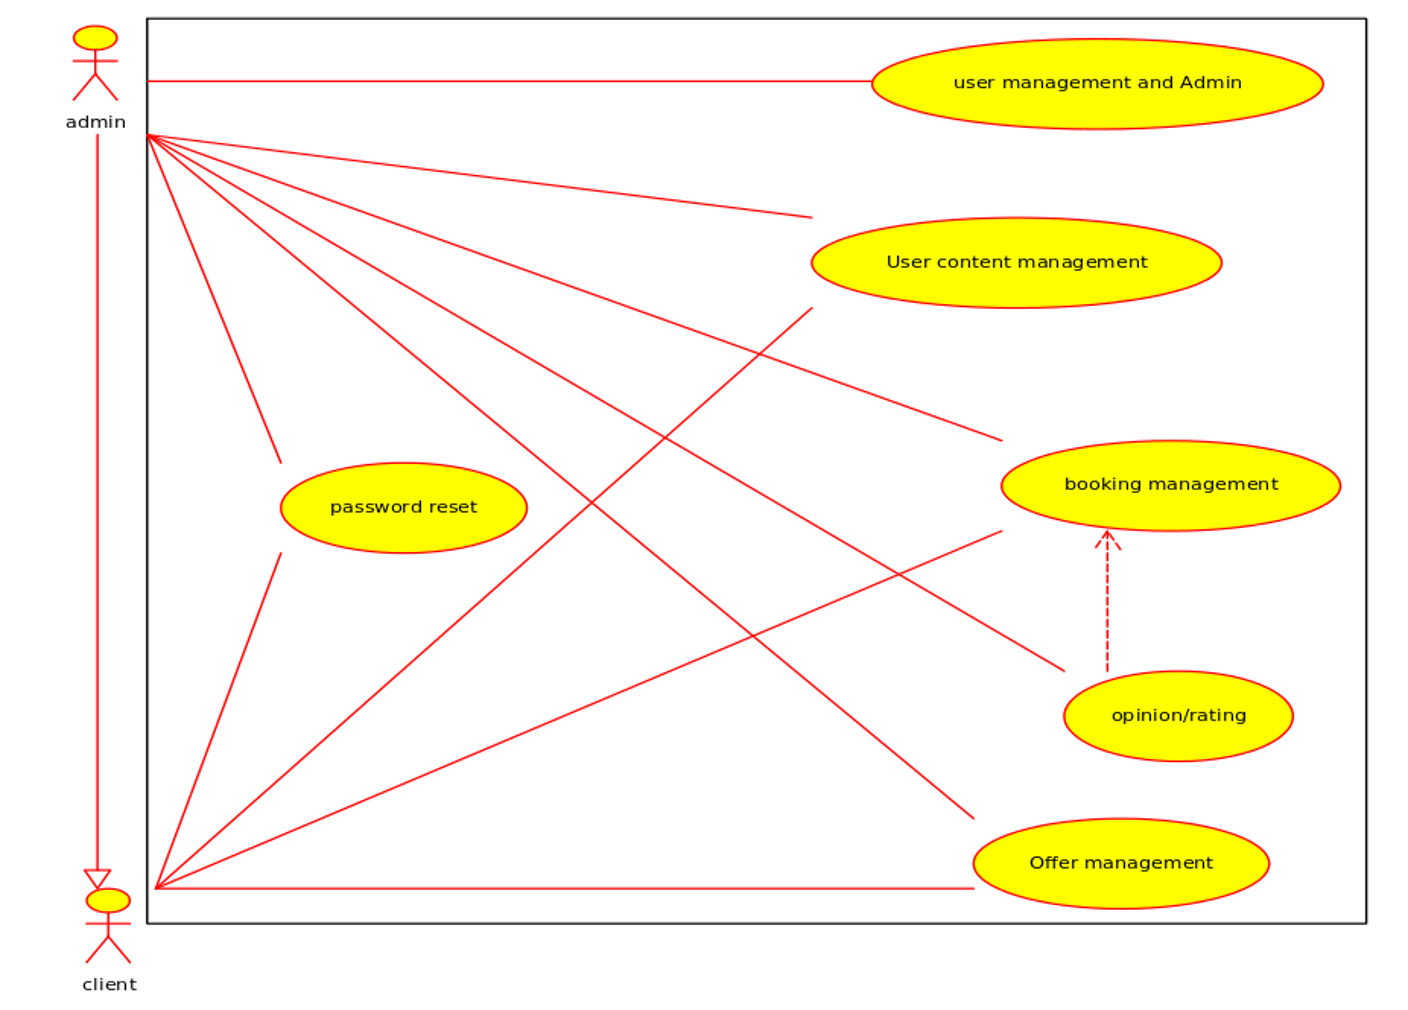
\includegraphics[scale=0.25]{img/updated_use_case.jpg}
\caption{Use case diagram}
\end{figure}
\subsection {User management}
\begin{itemize}
\item[1.] User selects action to preform on Users table on intended user
\item[2.] selecting create User a new screen appears:
	\begin{itemize}
		\item[a.] Admin enters details required to create user
		\item[b.] selects save option to save user or cancel to forget data
	\end{itemize}
\item[3.] selecting edit User, admin is presented with user details and proceeds as in \textbf{User Content Management}
\item[4.] selecting block
	\begin{itemize}
	\item[a.] Admin adds reason for blocking user
	\item[b.] confirms the block by selecting the save option
	\end{itemize}
\item[5.] Selecting unblock:
	\begin{itemize}
		\item[a.] Admin enters reason for unblocking user
		\item[b.] Selects the save option to confirm or cancel to forget action	
	\end{itemize}
\end{itemize}
\subsection {User Content Management}
\begin{itemize}
\item[1.] User selects profile settings attribute
\item[2.] List of user profile details is output to screen
\item[3.] User selects edit under selected profile attribute i.e name,surname,identity etc
\item[4.] User enters new parameter for selected attribute
\item[5.] User selects the save options to write the changes or cancel to ignore changes
\end{itemize}

\subsection {Offer Management}
\begin{itemize}
\item[1.] User selects the offers attribute 
\item[2.] User forwarded to search criteria page 
\item[3.] User is presented with options: Search,Add,Remove,Edit
\item[4.] User selects Search option:
	\begin{itemize}
		\item[a.] User presented with 'search bar' by system
		\item[b.] User enters search criteria: location of stay in the form of Country,city,region,street, date of arrival, date of departure, price ranges
		\item[c.] results output to screen
		\item[d.] selects offer of choice
		\item[e.] User presented with details of offer as entered by owner of the offer
		\item[f.] User proceeds to make booking as under \textbf{Booking Management}
	\end{itemize}
\item[5.]User selects Add option:
	\begin{itemize}
		\item[a.] System outputs a new options page
		\item[b.] User fills in offer details including : location of offer, number of people, price per night, additional options such as kitchen, bathroom, separate entrance etc
		\item[c.] User adds photos of the room on offer
		\item[d.] User saves the offer or presses cancel to forget
	\end{itemize}
\item[6.] User selects Remove option:
	\begin{itemize}
		\item[a.] User asked to confirm removal
		\item[b.] User confirms removal
		\item[c.] Offer removed from list of offers
	\end{itemize}
\item[7.] User selects Edit option:
	\begin{itemize}
		\item[a.] User presented with properties of offer
		\item[b.] User selects property intended for editing
		\item[c.] User enters new parameters for selected property
		\item[d.] User selects save to confirm changes or cancel to drop changes
	\end{itemize}
\end{itemize}
\subsection {Booking Management}
 \begin{itemize}
		\item[1.] Admin/Owner(user) select edit offer attribute
		\item[2.] user is presented with list of offer attributes
		\item[3.] user selects attribute to edit or offer to revoke
		\item[4.] user changes attribute accordingly if edit was selected
		\item[6.] user selects appropriate confirmation or cancel to ignore action
\end{itemize}
\subsection {Opinion Rating}
\begin{itemize}
\item[1.] User selects the rating attribute  rental
\item[2.] System outputs list of rating criteria onto screen
\item[3.] User enters rating for each criteria
\item[4.] User saves by confirming actions or cancels to forget
\end{itemize}
\section{Architecture}
\subsection{Representational State Transfer(ReST)}

\section{Class Diagrams}
\section{Database Design}
	\begin{figure}
		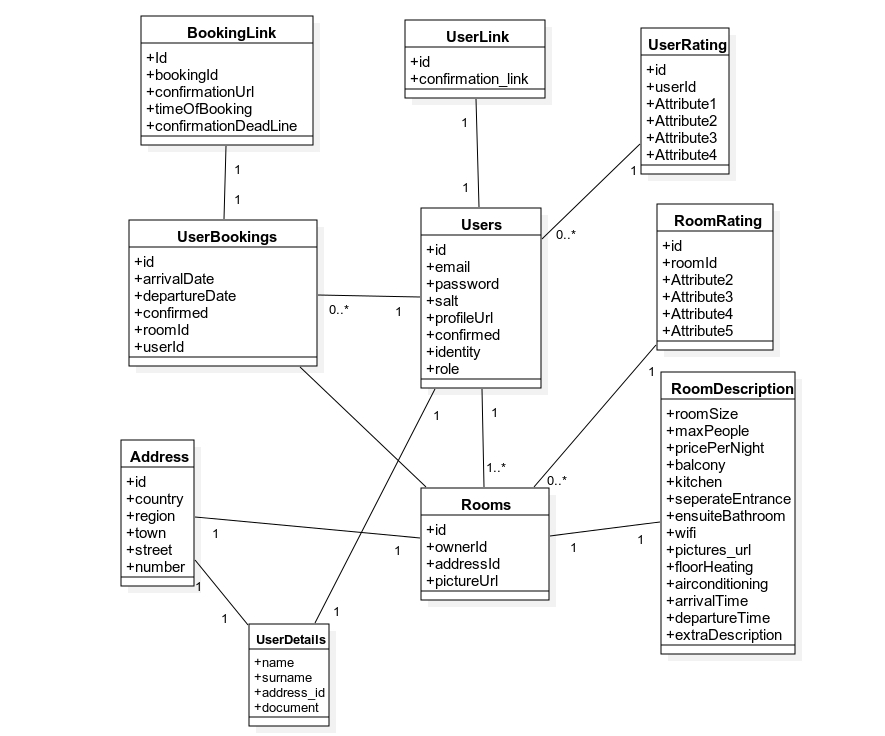
\includegraphics[scale=0.6]{./img/starUml.jpg} 
	\end{figure}
\section{Sequence Diagrams}
\section{Protocols}
\subsection*{Hypertext Transfer Protocol}

